\documentclass[border=5mm,tikz]{standalone}

\usetikzlibrary {3d} 

\begin{document}

\begin{tikzpicture}

\coordinate [label=120:0](zero) at (0,0,0);
\coordinate [label=120:x](x) at (7,0,0);
\coordinate [label=120:y](y) at (0,7,0);
\coordinate [label=120:z](z) at (0,0,7);

\coordinate [label=120:A](a) at (4,0,0);
\coordinate [label=270:B](b) at (4,4,0);
\coordinate [label=30:C](c) at (0,4,0);

\coordinate [label=120:H](h) at (0,0,6);
\coordinate [label=120:E](e) at (4,0,6);
\coordinate [label=240:F](f) at (4,4,6);
\coordinate [label=30:G](g) at (0,4,6);

\draw[dashed] (zero) -- (a);
\draw[dashed] (zero) -- (c);
\draw [dashed](zero) -- (h);

\draw (a) -- (b);
\draw (c) -- (b);
\draw (a) -- (x);
\draw (c) -- (y);

\draw (h) -- (z);
\draw (a) -- (e);
\draw (e) -- (h);
\draw (h) -- (g);
\draw (g) -- (f);
\draw (e) -- (f);
\draw (c) -- (g);
\draw (b) -- (f);
\end{tikzpicture}


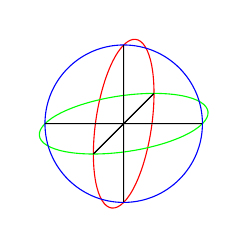
\begin{tikzpicture}
  \begin{scope}[canvas is zy plane at x=0]
    \draw [red] (0,0) circle (1cm);
    \draw (-1,0) -- (1,0) (0,-1) -- (0,1);
  \end{scope}

  \begin{scope}[canvas is zx plane at y=0]
    \draw [green] (0,0) circle (1cm);
    \draw (-1,0) -- (1,0) (0,-1) -- (0,1);
  \end{scope}

  \begin{scope}[canvas is xy plane at z=0]
    \draw[blue] (0,0) circle (1cm);
    \draw (-1,0) -- (1,0) (0,-1) -- (0,1);
  \end{scope}
\end{tikzpicture}


\end{document}
